Neuschnee verändert sich durch eine Schneemetamorphose. Bei der Metamorphose sublimiert Eis zu Wasserdampf und lagert sich an einer anderen Stelle wieder an. Die Geschwindigkeit dieser Umwandlung variiert je nach Umgebungsbedingungen stark. Die Temperatur im Schnee bleibt dabei relativ konstant bei 0 Grad Celsius.

Während der Metamorphose ändern sich die Eigenschaften des Schnees. Ein grundlegendes Prinzip bei der Metamorphose ist das Bestreben, die Oberfläche zu verkleinern, was bedeutet, dass feine Eisästchen in konkave Mulden umgewandelt werden. Dieser Prozess ist ein Beispiel für Energieoptimierung, da das System bestrebt ist, einen energetisch günstigeren Zustand zu erreichen.

Bei der Schmelzmetamorphose bildet sich Schmelzwasser im Porenraum des Schnees. Die Umwandlung zu runden Strukturen schreitet dabei besonders schnell voran. \cite{WSLSLFMetha.2024}

\begin{figure}[H]
    \centering
    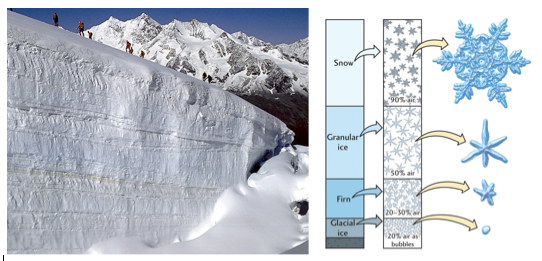
\includegraphics[width=0.9\textwidth]{Bilder/gletscher_eis_schnee.png}
    \caption{Darstellung der Schneemetamorphose, Bild aus \cite{Wetterdienst.6222017}}
    \label{fig:Metha}
\end{figure}
